\documentclass[11pt,a4paper]{article}
\usepackage[T1]{fontenc}
\usepackage{textcomp}
\usepackage{tgtermes}
\usepackage{tgheros}
\usepackage[english]{babel}
\babelprovide[import, main, hyphenrules=nohyphenation]{french}
\emergencystretch=3em
\usepackage[a4paper,margin=2.2cm]{geometry}
\usepackage{graphicx}
\usepackage{booktabs}
\usepackage{tabularx}
\usepackage{float}
\usepackage[font=small,labelfont=bf]{caption}
\usepackage{microtype}
\usepackage[hidelinks]{hyperref}
\usepackage{enumitem}
\setlist{itemsep=2pt,topsep=3pt}
\graphicspath{{../../figures/}}
\newcommand{\NOx}{NO\textsubscript{x}}
\newcommand{\NOd}{NO\textsubscript{2}}
\newcommand{\SOd}{SO\textsubscript{2}}
\newcommand{\ugm}{µg/m\textsuperscript{3}}
\newcommand{\zz}{z\textsubscript{0}}
\newcolumntype{Y}{>{\raggedright\arraybackslash}X}

\title{Dispersion des \NOx{} de la verrerie O-I de Reims en 2024 :\\modélisation AERMOD et confrontation aux mesures}
\author{Mahamat Ali Ousmane\\{\small ORCID 0009-0009-6013-2834}}
\date{Novembre 2026 — version 1.0}

\begin{document}
\renewcommand{\tablename}{Tableau}\captionsetup{labelsep=period}
\maketitle

\begin{abstract}
\noindent Ce travail personnel estime, avec le modèle réglementaire AERMOD de l'US EPA, la contribution de la verrerie
O-I France, premier émetteur de \NOx{} de l'agglomération de Reims (143~t en 2024), au \NOd{} mesuré par les trois
stations d'ATMO Grand Est. La contribution annuelle de l'usine aux stations est de 0,03 à 0,05~\ugm{} de \NOd{} avec
l'option rurale d'AERMOD et de 0,05 à 0,13~\ugm{} avec l'option urbaine, soit moins de 0,5~\% à 1,4~\% du \NOd{}
mesuré. Le choix entre ces deux options, que les critères de l'EPA ne tranchent pas ici, est le premier facteur
d'incertitude. Aucun autre facteur testé ne change l'ordre de grandeur~: météo simulée à 1~km par WRF en janvier
et en juillet, rugosité du site, rayonnement, brouillard, fumigation, paramètres de la cheminée. Treize ans de
mesures, pendant lesquels les émissions ont varié d'un facteur~4, défavorisent l'option urbaine sans la réfuter~:
le signal de l'usine est 10 à 100 fois plus petit que la variabilité mesurée, et le réseau ne peut pas le
détecter. \textit{Il s'agit d'un exercice d'apprentissage et non d'une expertise réglementaire.}
\end{abstract}

\section{Question et cadre}
La verrerie O-I France (bouteilles en verre, deux fours, cheminée unique de 59~m) est le plus gros émetteur de
\NOx{} de l'agglomération rémoise, couverte par un plan de protection de l'atmosphère où le \NOx{} est le polluant
le plus problématique. Deux questions guident ce travail~:
\begin{enumerate}
\item quelle part du \NOd{} mesuré aux stations de Reims provient de la verrerie~?
\item le réseau de mesure permet-il de mettre cette contribution en évidence~?
\end{enumerate}
L'étude utilise uniquement des données publiques et des hypothèses documentées. Elle n'a été ni vérifiée ni
validée par l'exploitant ou par l'administration. Les calculs, les entrées et les scripts sont dans le dépôt
associé (§~\ref{sec:repro}).

\section{Installation et données}
\begin{table}[htbp]
\centering\small
\caption{Paramètres de la source retenus.}
\begin{tabularx}{\textwidth}{lY}
\toprule
Paramètre & Valeur et origine \\
\midrule
Cheminée & unique (fours 2 et 3), 59~m, diamètre 2,51~m (arrêté préfectoral 2025-APC-277-IC) \\
Fumées & 523~K, 8~m/s (vitesse minimale prescrite) \\
Position & triangulation sur Street View et orthophotographie IGN (UTM 31N~: 576\,601~m E, 5\,453\,845~m N) \\
Émissions & 143~t de \NOx{} en 2024 (IREP), soit 4,5~g/s, modulées par mois selon la production (arrêt du four~3 le 12/07) \\
Bâtiments & 599 bâtiments de plus de 3~m (BD TOPO), sillage calculé par BPIPPRM \\
\bottomrule
\end{tabularx}
\end{table}

\begin{table}[htbp]
\centering\small
\caption{Données utilisées.}
\begin{tabularx}{\textwidth}{lY}
\toprule
Donnée & Source et traitement \\
\midrule
Météo de surface & Reims-Prunay (NOAA ISD), à 7~km à l'est-sud-est~; nébulosité «~CAVOK~» mise à 0 octa (contrôlé par l'ensoleillement mesuré)~; 381~heures manquantes complétées par la base horaire Météo-France \\
Radiosondages & Trappes, secours Idar-Oberstein (IGRA2) \\
Relief & IGN RGE ALTI 25~m~; grille de 81 × 81 récepteurs au pas de 250~m (20 × 20~km) \\
Occupation du sol & Corine Land Cover 2018~; logements BD TOPO \\
Mesures & \NOd, NO, \NOx{} et O\textsubscript{3} horaires validés 2024 (LCSQA, ATMO Grand Est), stations Jean d'Aulan (fond urbain, 2,5~km), Doumer (trafic, 2,9~km), Bétheny (fond périurbain, 5,5~km)~; \NOd{} 2013–2025 (AEE) \\
Météo simulée & WRF 4.7.1 forcé par ERA5, domaines 9/3/1~km, janvier et juillet 2024~; MMIF 4.1.1 \\
\bottomrule
\end{tabularx}
\end{table}

\begin{figure}[htbp]
\centering
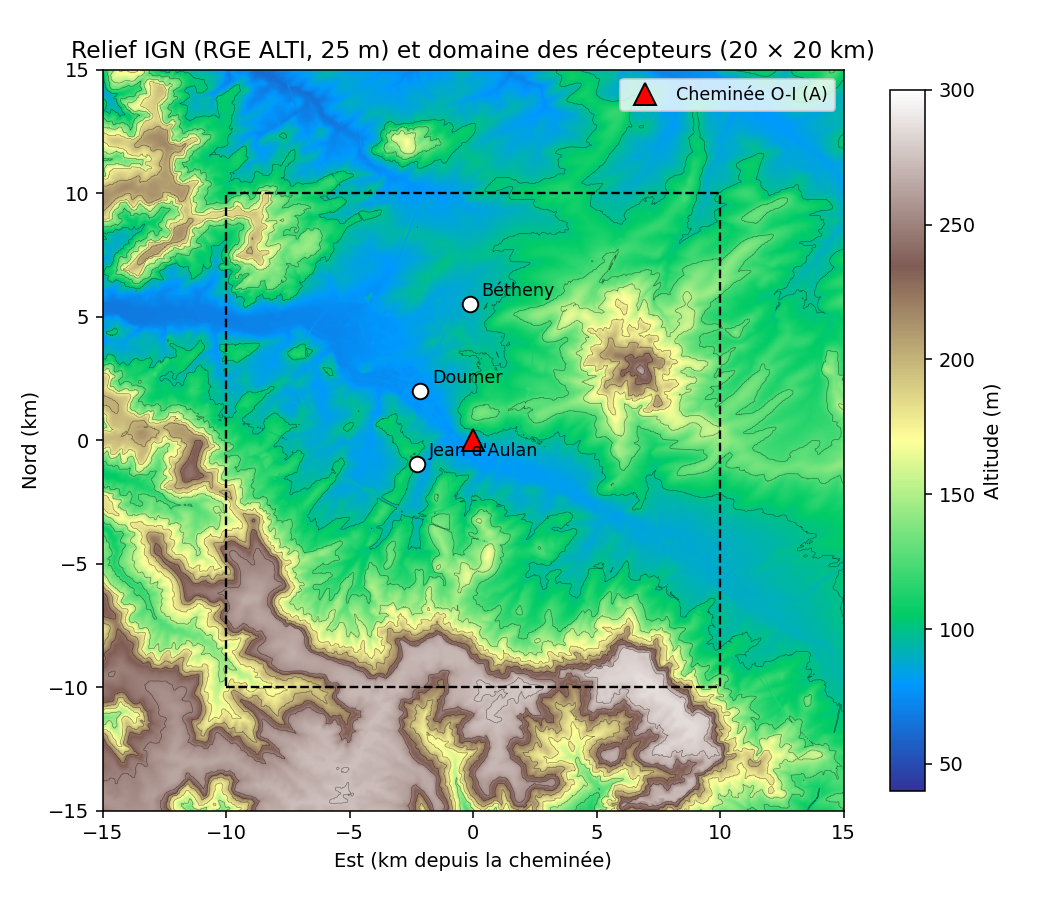
\includegraphics[width=0.62\textwidth]{relief_recepteurs.png}
\caption{Relief autour de la verrerie et domaine des récepteurs. Le Mont de Berru (est) et la Montagne de Reims
(sud) dominent la plaine de 100 à 200~m.}
\end{figure}

\section{Méthode}
\textbf{Météo.} AERMET traite la météo de Prunay avec les caractéristiques de surface du site de mesure, comme le
demande l'EPA pour un vent mesuré (champs~: \zz{} de 0,03~m en hiver à 0,15~m en été). L'option de correction de
u\textsuperscript{*} par vent faible et stable (ADJ\_U*) est activée. 98 à 100~\% des heures sont utilisables.

\textbf{Rural ou urbain.} AERMOD traite différemment la couche limite nocturne en ville. Les deux critères de l'EPA
se contredisent ici~: la méthode d'Auer (1978), fondée sur l'occupation du sol dans un rayon de 3~km, donne
\emph{rural} (24~\% de sols urbains), alors que la densité de population (environ 3\,000~hab/km², pour un seuil de
750) donne \emph{urbain}. Les résultats sont donc donnés en fourchette~: option rurale (référence) et option urbaine
(population de 182\,000~habitants, borne haute).

\textbf{Conversion en \NOd.} Les méthodes OLM et ARM2 donnent toutes deux \NOd{}~=~0,9 × \NOx{} à toutes les
heures~: l'ozone mesuré (52~\ugm{} en moyenne) est toujours en excès devant le \NOx{} de l'usine.

\textbf{Confrontation aux mesures.} Trois tests~: moyennes par secteur de vent en 2024~; «~expérience naturelle~»
2013–2025, qui exploite la variation d'un facteur~4 des émissions déclarées (143 à 566~t/an)~; régression horaire
du \NOx{} mesuré sur la contribution modélisée, avec effets de l'heure du jour et de la vitesse du vent.

\textbf{Météo simulée.} Pour tester la représentativité de Prunay, WRF a été exécuté à 1~km sur janvier et juillet
2024. MMIF extrait la maille de la cheminée et prépare les entrées d'AERMET.

\section{Résultats 2024}
\begin{table}[htbp]
\centering\small
\caption{Contribution de la verrerie en 2024 (bâtiments inclus).}
\begin{tabular}{lcc}
\toprule
Indicateur & Rural (référence) & Urbain (borne haute) \\
\midrule
Moyenne annuelle maximale (\NOx), à 0,7~km au nord-est & 0,22~\ugm & 0,28~\ugm \\
Maximum horaire (\NOx) & 49~\ugm{} (Mont de Berru) & 14~\ugm \\
Moyenne annuelle aux 3 stations (\NOd) & 0,03 à 0,05~\ugm & 0,05 à 0,13~\ugm \\
Part du \NOd{} mesuré aux stations & < 0,5~\% & 0,5 à 1,4~\% \\
\bottomrule
\end{tabular}
\end{table}

\begin{figure}[htbp]
\centering
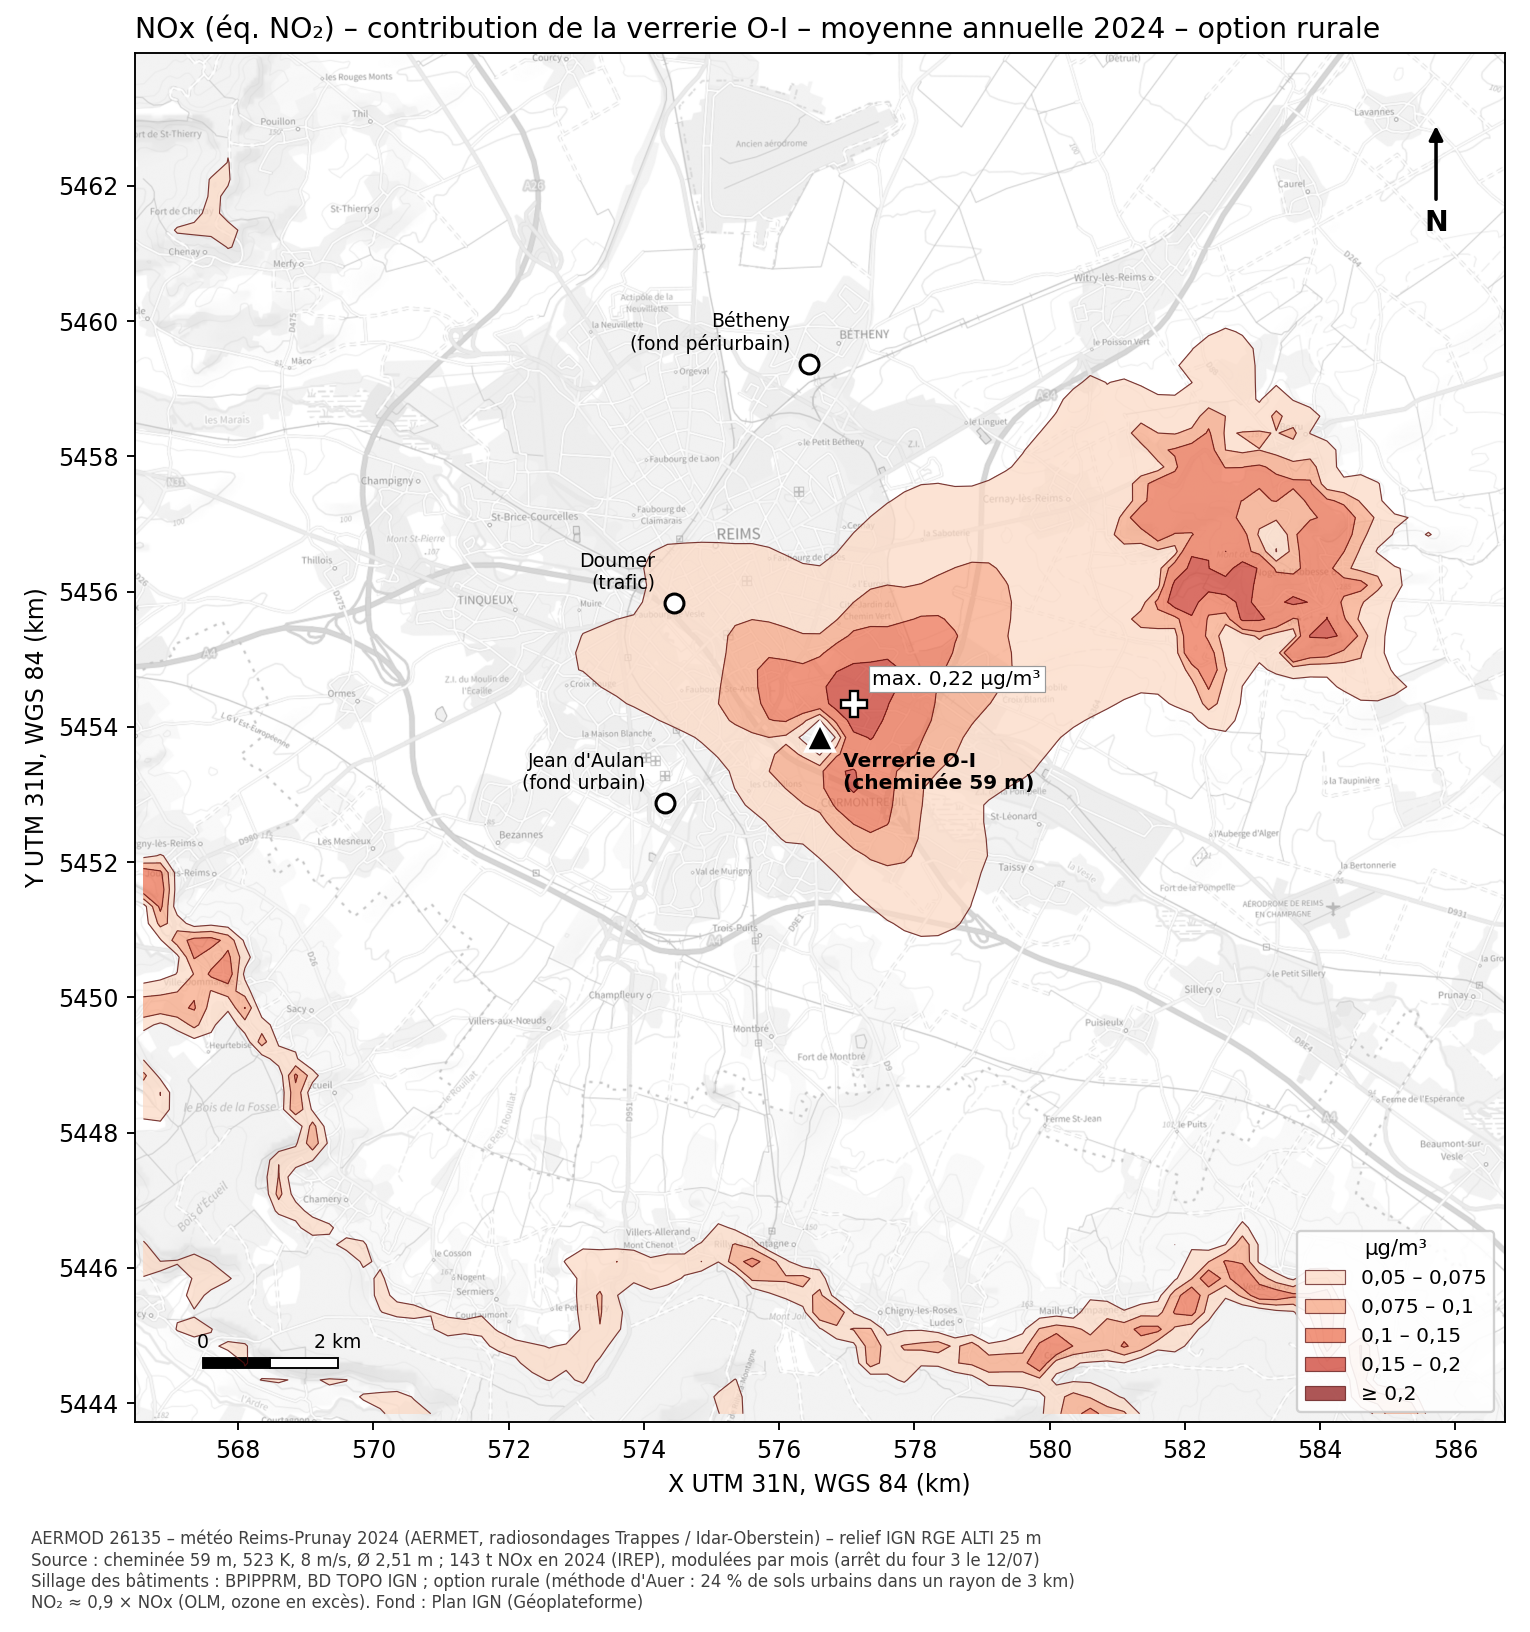
\includegraphics[width=0.49\textwidth]{aermod_rural_2024_annuel.png}\hfill
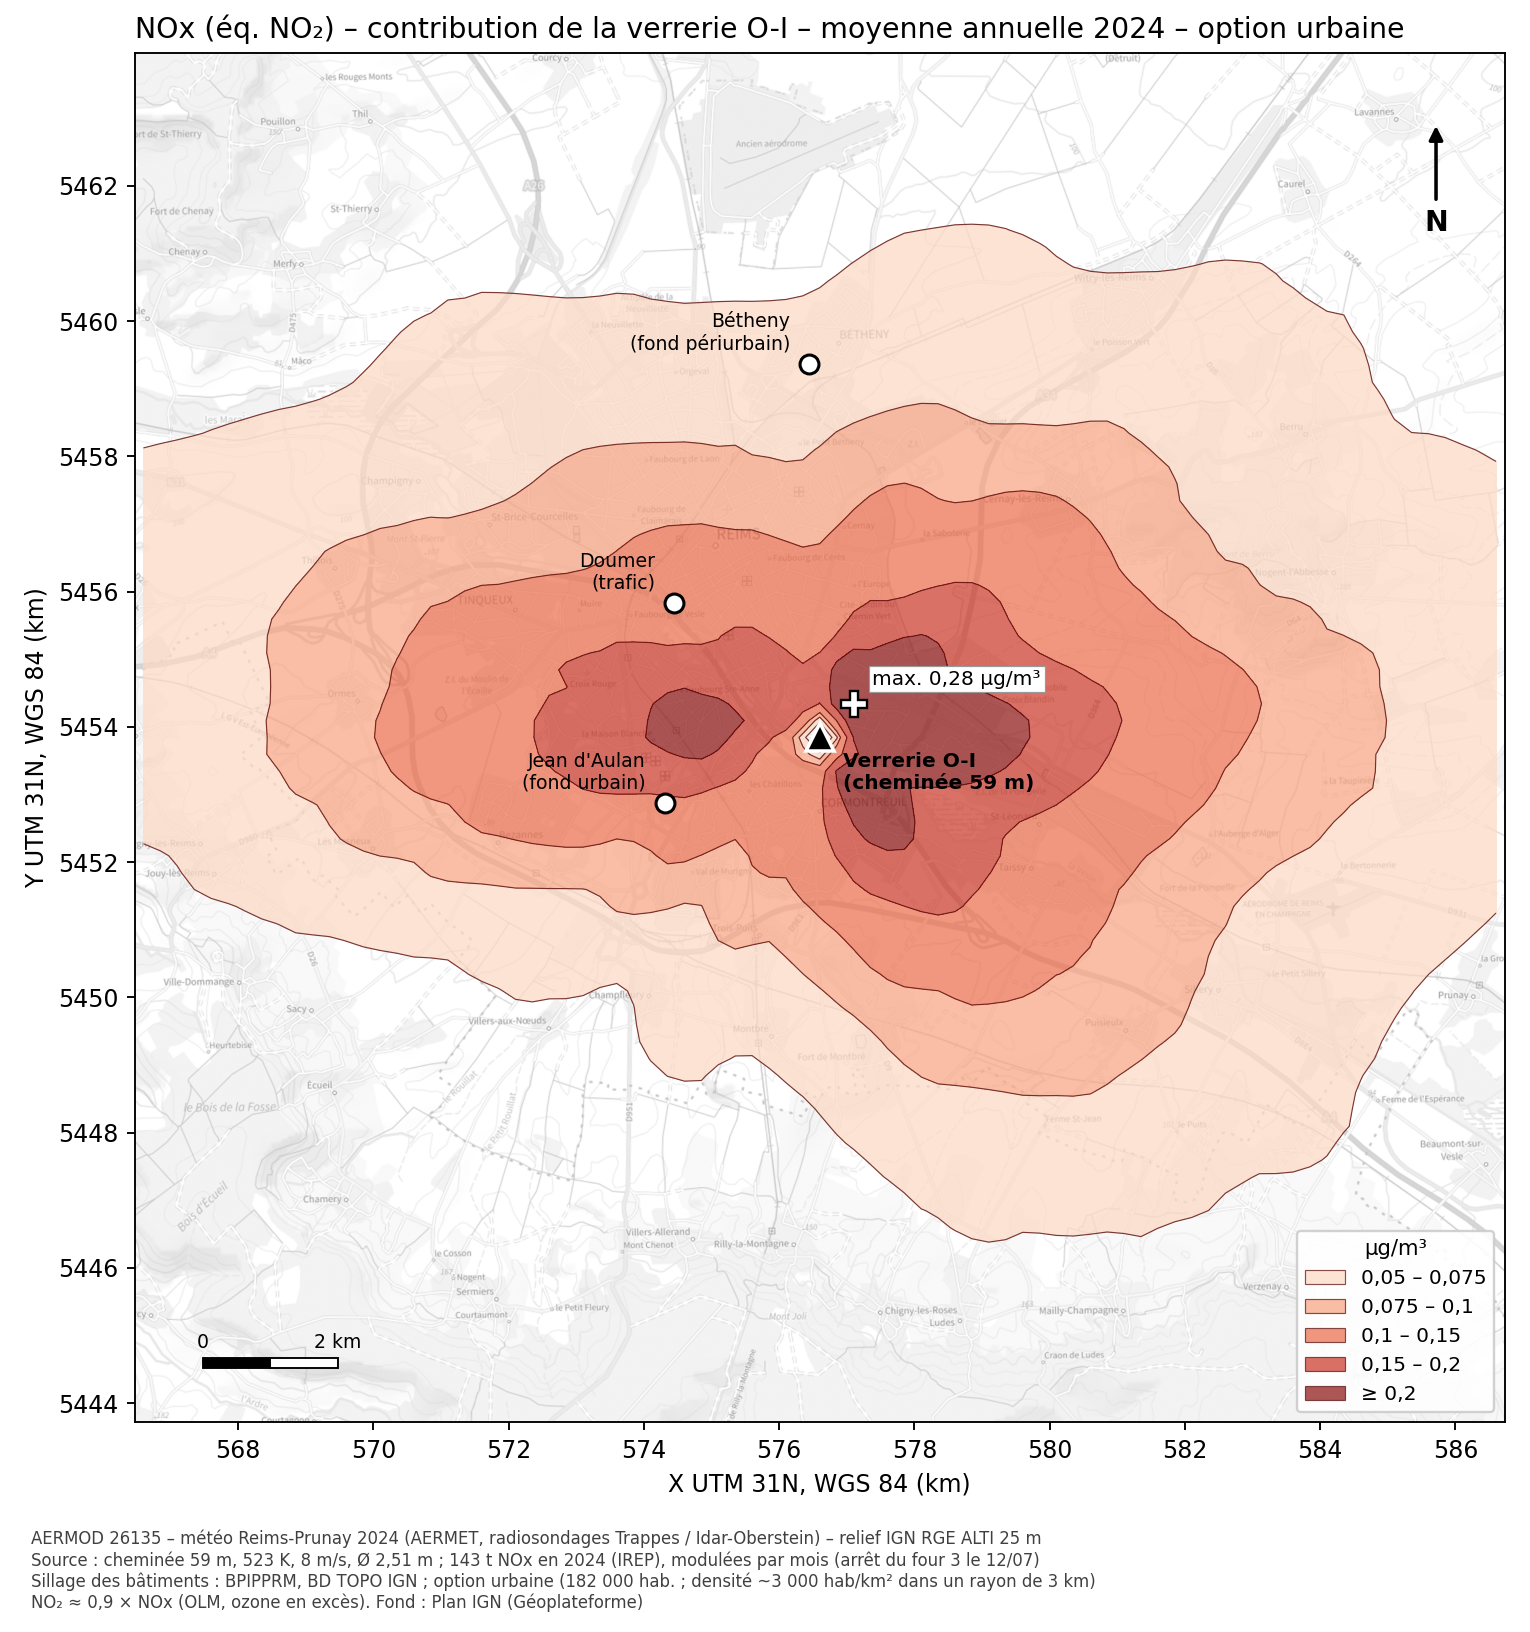
\includegraphics[width=0.49\textwidth]{aermod_reference_2024_annuel.png}
\caption{Moyenne annuelle 2024 de la contribution de l'usine (\NOx), option rurale (gauche) et urbaine (droite),
avec les mêmes classes. Rien n'est coloré sous 0,05~\ugm.}
\end{figure}

Le panache part surtout vers le nord-est, sous les vents dominants de sud-ouest. En option rurale, il touche aussi
le relief à 6–7~km (Mont de Berru) et les pentes de la Montagne de Reims. L'option urbaine donne une tache plus
étendue et plus symétrique, avec un lobe vers l'ouest qui passe sur Jean d'Aulan et Doumer~: c'est pourquoi elle
donne 2 à 4 fois plus aux stations, alors que son maximum n'est guère plus fort. Aucune des deux options n'est la
plus prudente partout~: l'urbaine donne davantage en moyenne annuelle, la rurale en maximum horaire, à cause du
relief (fig.~\ref{fig:max1h}).

\begin{figure}[htbp]
\centering
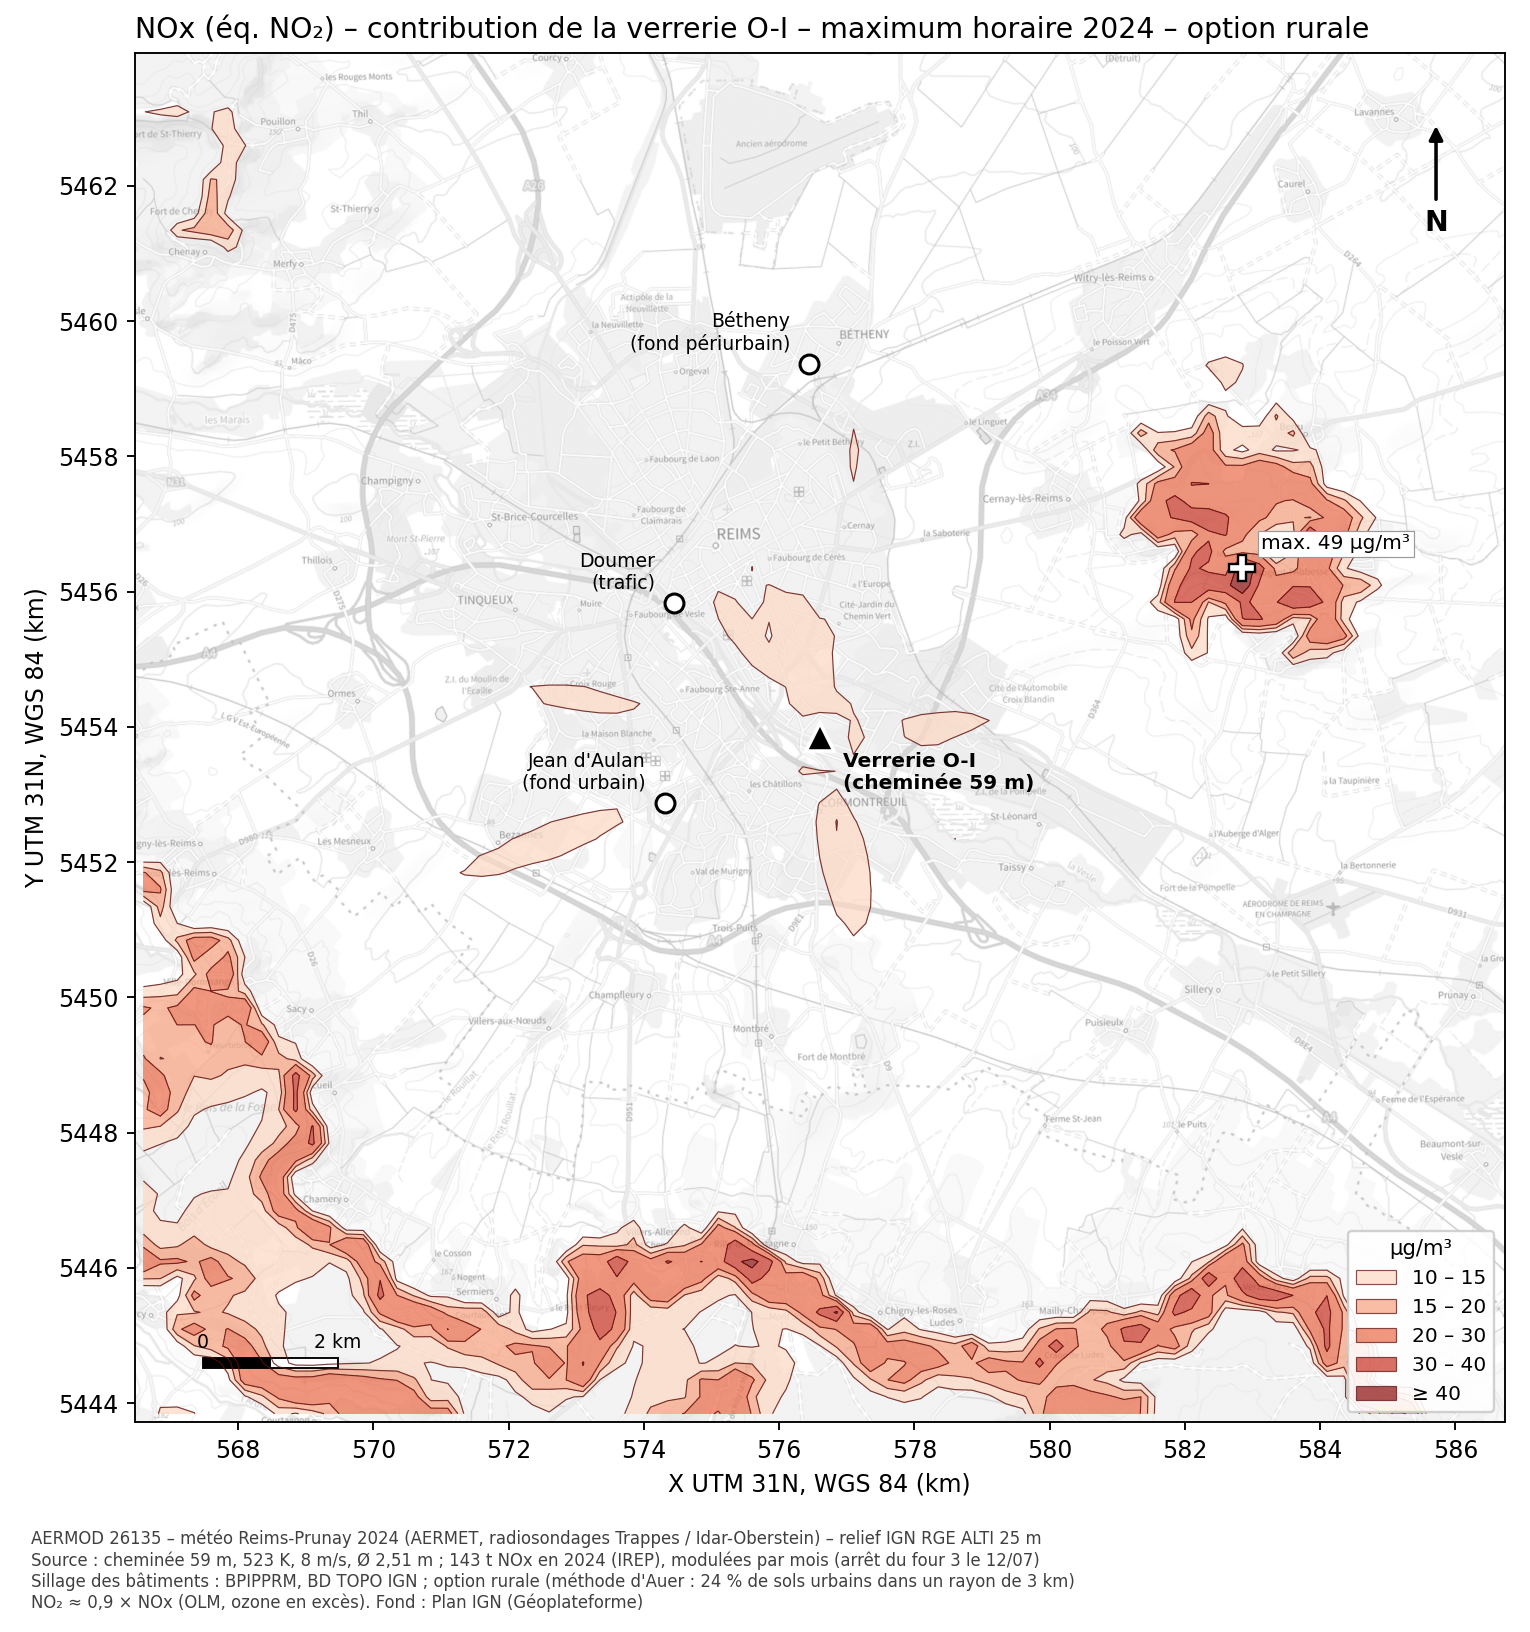
\includegraphics[width=0.49\textwidth]{aermod_rural_2024_max1h.png}\hfill
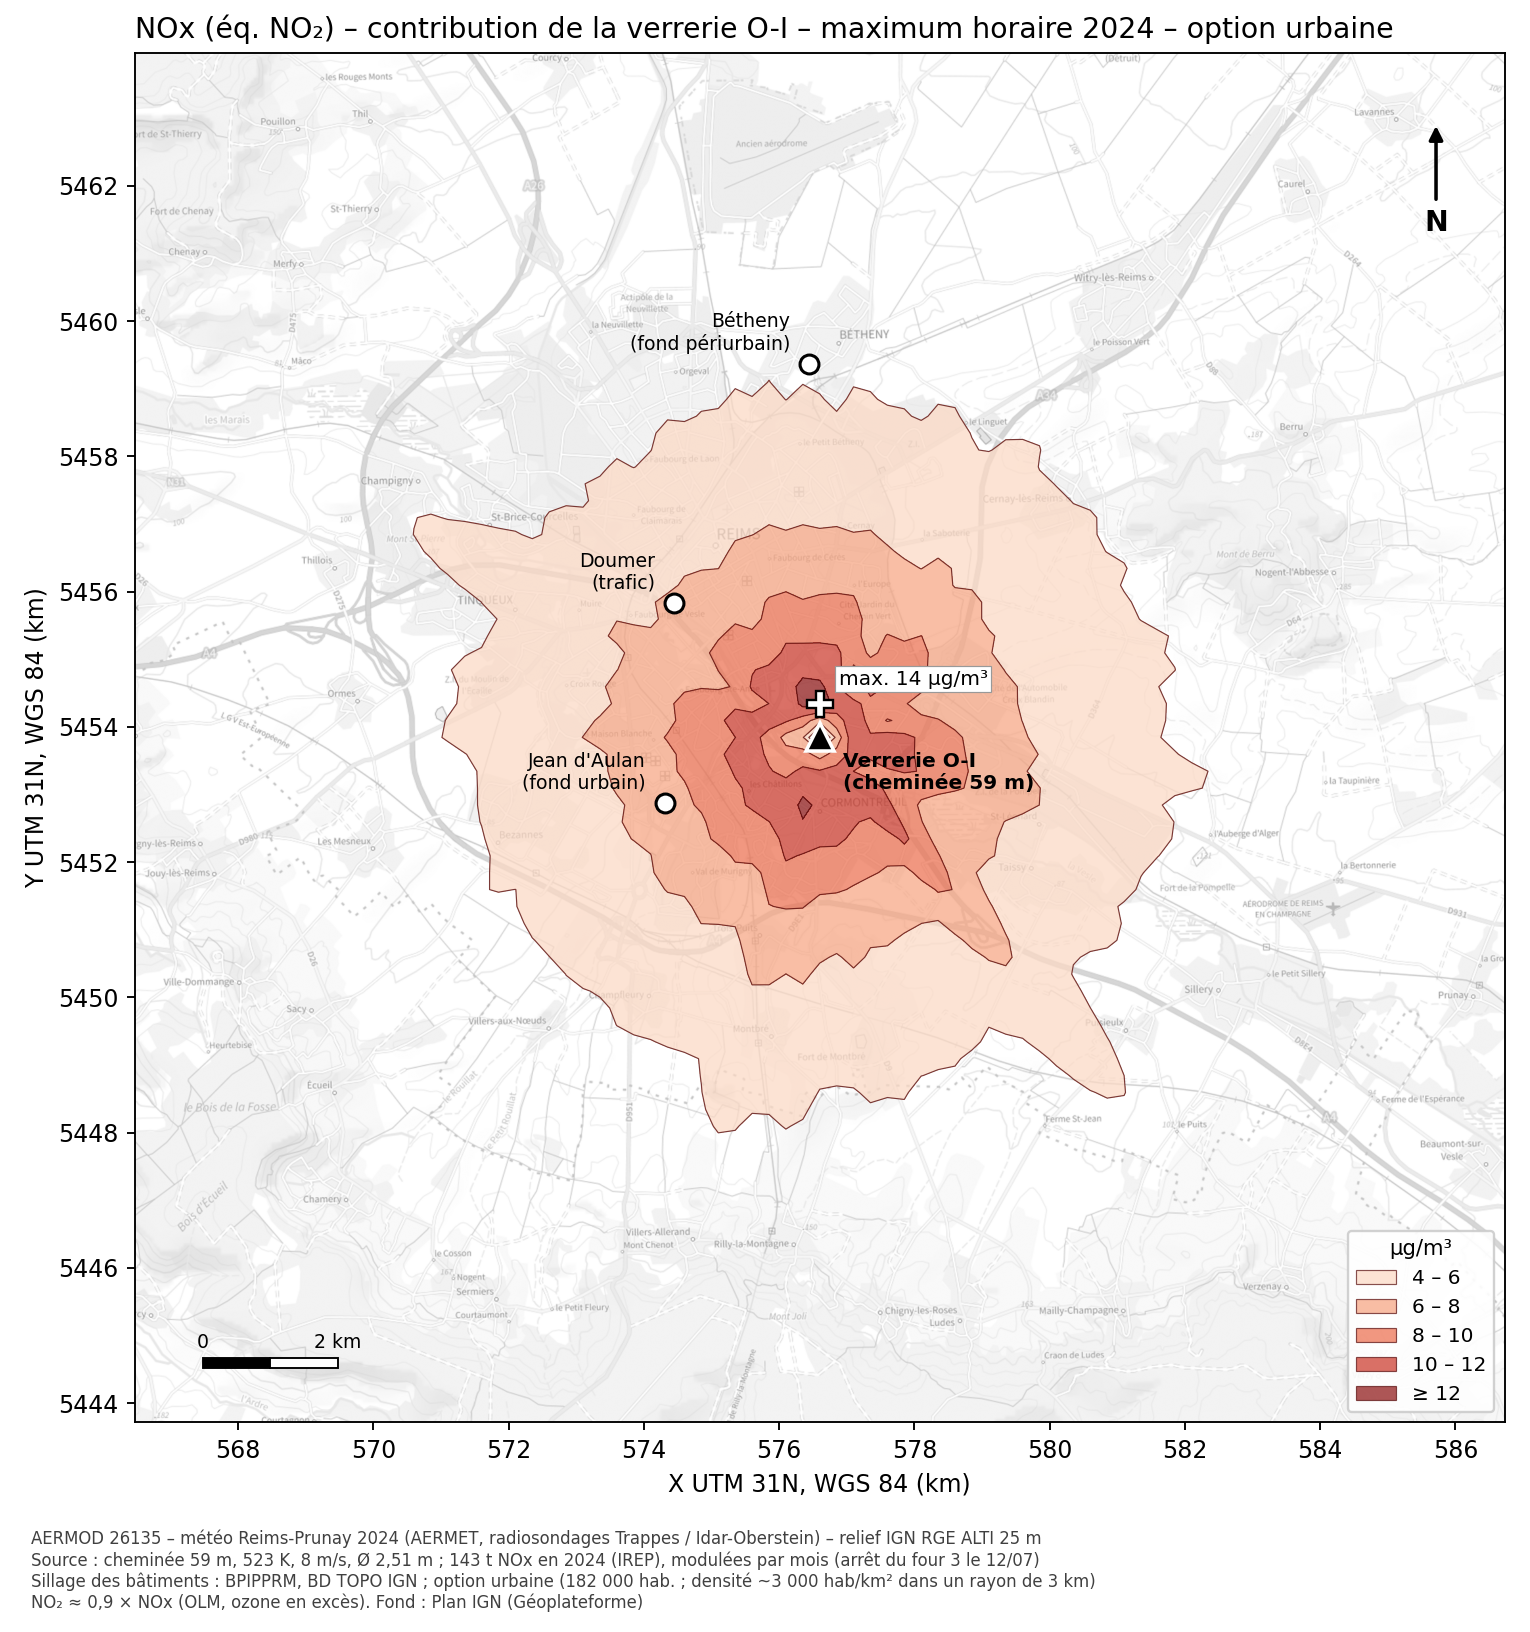
\includegraphics[width=0.49\textwidth]{aermod_reference_2024_max1h.png}
\caption{Maximum horaire 2024 (\NOx), option rurale (gauche, 49~\ugm{} sur le Mont de Berru) et urbaine (droite,
14~\ugm). Chaque carte a ses propres classes~: comparer les valeurs, pas les couleurs.}
\label{fig:max1h}
\end{figure}

\section{Confrontation aux mesures}
\textbf{Par secteur de vent.} Le modèle place l'influence de l'usine dans un pic étroit (±\,15°) dans la direction
de la verrerie vue de chaque station. En moyenne sur ce secteur, la contribution modélisée est de 0,3 à 0,5~\ugm{}
de \NOd{} en option rurale et de 0,7 à 1,6~\ugm{} en option urbaine, soit 2 à 11~\% du \NOd{} mesuré dans
le même secteur. Les mesures ne montrent pas ce pic~: les variations
du \NOd{} avec la direction du vent (facteur 2 à 3) suivent les situations météorologiques. Les vents de nord-est,
froids et stables, donnent le \NOd{} le plus élevé aux trois stations à la fois, y compris là où l'usine n'est
pas dans cette direction (fig.~\ref{fig:secteurs}).

\begin{figure}[htbp]
\centering
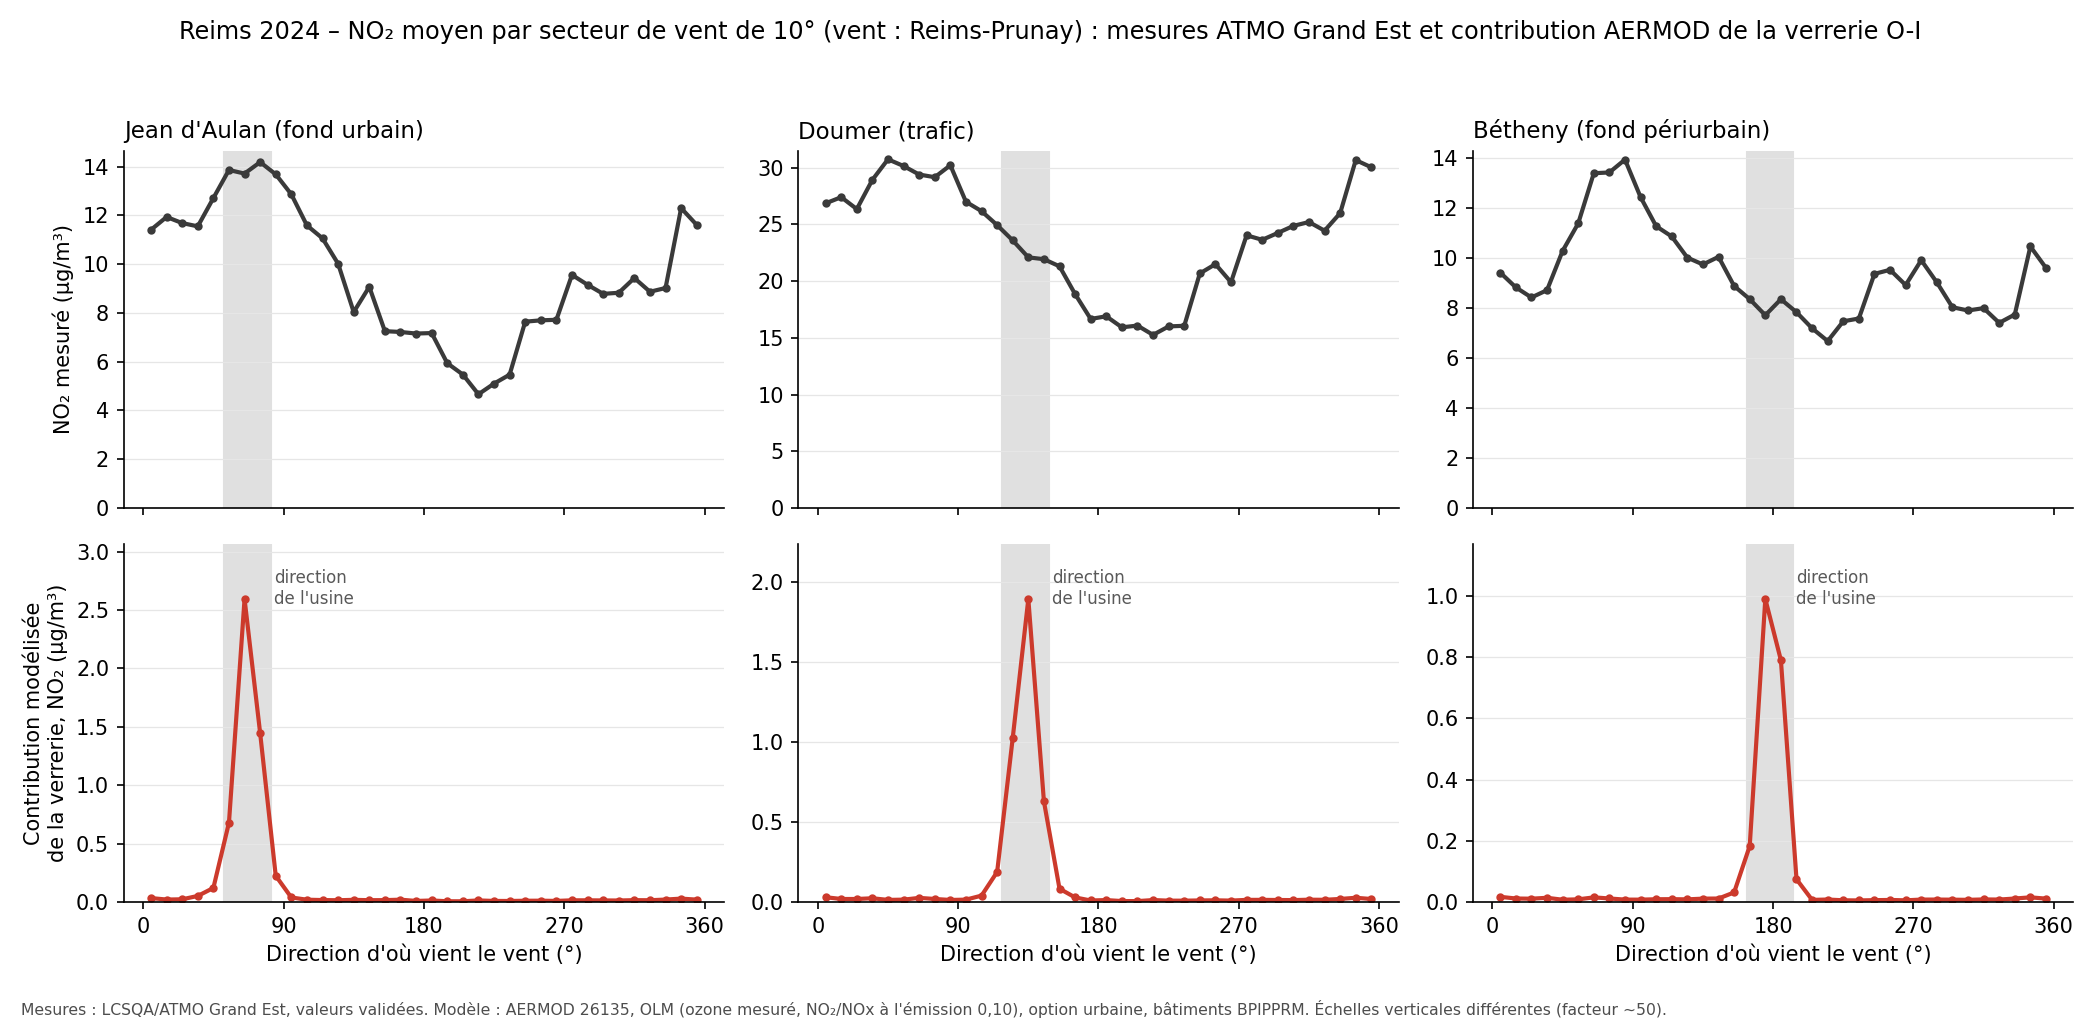
\includegraphics[width=\textwidth]{etape6_secteurs_no2.png}
\caption{\NOd{} moyen par secteur de vent de 10° en 2024~: mesures (haut) et contribution modélisée de la verrerie,
option urbaine (bas~; échelles différentes d'un facteur 50 environ). Bande grise~: direction de l'usine.}
\label{fig:secteurs}
\end{figure}

\textbf{Expérience naturelle 2013–2025.} Si l'usine contribuait notablement, l'excès de \NOd{} par vent venant de
l'usine (par rapport aux secteurs voisins) suivrait ses émissions annuelles. On mesure la pente de cet excès en
fonction des émissions, rapportée à la pente prévue par AERMOD ($\beta = 1$ si le modèle est juste, $\beta = 0$ si
l'usine n'a pas d'effet visible). Si la direction du vent de Prunay était exacte, on obtiendrait
$\beta = -0{,}16 \pm 0{,}22$ pour l'option urbaine et $\beta = -0{,}08 \pm 0{,}65$ pour l'option rurale
(fig.~\ref{fig:exp}). Mais l'écart de direction entre le vent de Prunay et celui de WRF à la maille de l'usine a un
écart type robuste de 26° en janvier et de 38° en juillet. Avec une erreur de direction de 20 à 40°, l'option
urbaine n'est plus défavorisée qu'à 1,1 à 2,2 écarts types, et l'option rurale reste compatible. Le test indique une
préférence~; il ne tranche pas.

\begin{figure}[htbp]
\centering
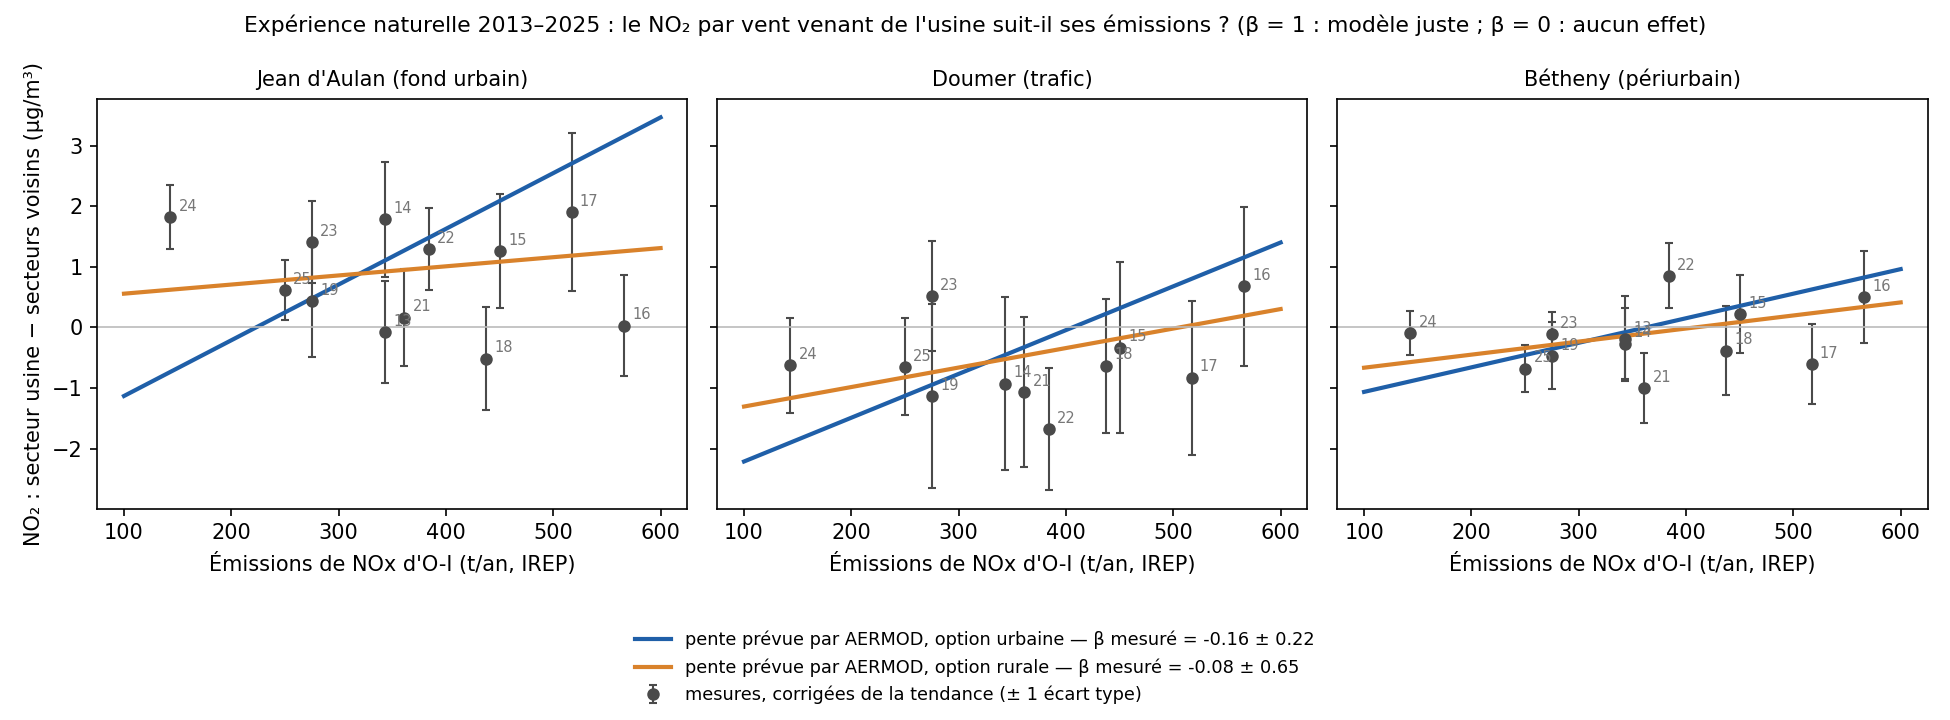
\includegraphics[width=\textwidth]{etape6_experience_naturelle.png}
\caption{Excès de \NOd{} par vent venant de l'usine en fonction des émissions annuelles d'O-I, 2013–2025, et pentes
prévues par AERMOD (direction du vent supposée exacte).}
\label{fig:exp}
\end{figure}

\textbf{Heure par heure.} Sans contrôle, la corrélation de rang entre le \NOx{} mesuré et la contribution modélisée
vaut $-0{,}3$ à $-0{,}4$ en option rurale et $+0{,}3$ à $+0{,}4$ en option urbaine (janvier). Le signe dépend de
l'option, pas de l'usine. En rural, le panache atteint les stations par vent soutenu, quand l'air urbain est propre~;
en urbain, il les atteint par temps calme, quand le \NOx{} du trafic s'accumule. Une fois l'heure du jour et la
vitesse du vent prises en compte, la pente $\beta$ n'est pas mesurable~: ses écarts types vont de 0,45 à 24 sur
42 régressions (7 cas, 3 stations, 2 mois). Le signal de l'usine (0,3 à 4,6~\ugm{} au 99\textsuperscript{e}
centile horaire) est noyé dans des variations horaires de 5 à 63~\ugm.

\textbf{Îlot de chaleur de l'usine.} Paine et al. (2016) justifient l'option urbaine près d'une grande usine si elle
crée un îlot de chaleur d'au moins 8~K sur quelques centaines de mètres. Sur 32 images Landsat sans nuages, l'usine
a une signature thermique propre mais modérée~: +1,7~K en moyenne dans 300~m en hiver, et aucun pixel au-dessus de
+8~K. Sur 9 nuits ASTER, elle ne se distingue pas du tissu urbain~: +1,2~K en moyenne, et aucun pixel au-dessus de
+4~K. Le critère n'est pas atteint, ce qui ne justifie pas l'option urbaine par un effet propre à l'usine.

\section{Météo simulée par WRF}
Prunay est à 7~km, en campagne. WRF a donc été exécuté à 1~km de résolution, et AERMOD relancé avec la météo de la
maille de la cheminée. Selon l'EPA (guide MMIF, § 3.3), il faut alors utiliser les caractéristiques de surface de la
maille du modèle, fournies par MMIF. La maille de 1~km est classée «~urbaine~», avec \zz{}~=~0,8~m. Or Corine montre
que le kilomètre autour de la cheminée est à moitié ouvert ou boisé~: 32~\% de tissu urbain discontinu, 14~\% de
zones industrielles, 19~\% de cultures, 17~\% d'espaces de sport et loisirs, 12~\% de forêt et 7~\% de vignes. Une
variante avec \zz{}~=~0,25~m estimé à partir de ces classes a donc été ajoutée.

\begin{table}[htbp]
\centering\small
\caption{Contribution moyenne du mois (\NOx, \ugm) aux stations Jean d'Aulan / Doumer / Bétheny.}
\begin{tabular}{lcc}
\toprule
Météo, option & Janvier 2024 & Juillet 2024 \\
\midrule
Prunay, rural (référence) & 0,025 / 0,029 / 0,044 & 0,057 / 0,073 / 0,024 \\
Prunay, urbain & 0,195 / 0,115 / 0,078 & 0,142 / 0,130 / 0,055 \\
WRF, surface MMIF (\zz{} 0,8~m), rural & 0,115 / 0,164 / 0,054 & 0,050 / 0,042 / 0,019 \\
WRF, surface MMIF, urbain & 0,222 / 0,237 / 0,077 & 0,106 / 0,127 / 0,035 \\
WRF, \zz{} 0,25~m, rural & 0,058 / 0,078 / 0,055 & 0,054 / 0,048 / 0,018 \\
WRF, \zz{} 0,25~m, urbain & 0,183 / 0,255 / 0,085 & 0,109 / 0,144 / 0,038 \\
\bottomrule
\end{tabular}
\end{table}

\begin{itemize}
\item \textbf{En hiver}, la rugosité fait tout. Avec \zz{}~=~0,8~m, la turbulence mécanique de WRF rabat le panache
près de la source~: maximum mensuel de 1,8~\ugm{} à 0,4~km, et × 1,2 à × 5,7 aux stations par rapport à Prunay.
Avec \zz{}~=~0,25~m, on obtient × 1,2 à × 2,7.
\item \textbf{En été}, la convection domine (couche mélangée de 700 à 1\,000~m le jour)~: WRF redonne aux stations
les valeurs de Prunay (× 0,6 à × 1).
\item \textbf{Rugosité forte.} Des tests à \zz{}~=~1, 1,5 et 2~m donnent au plus 0,17~\ugm{} aux stations en option rurale. Au-delà
de \zz{} $\approx$ 1,4~m, AERMET n'accepte plus le vent à 10~m comme vent de référence~: celui-ci doit être mesuré
à au moins 7\,\zz{} (guide AERMET). La réponse devient alors irrégulière. Avec un vent mesuré à 10~m seulement,
AERMOD ne peut donc pas traiter une rugosité de centre-ville.
\end{itemize}
Dans tous les cas, la contribution aux stations reste d'au plus 0,26~\ugm{} sur le mois~: la météo simulée ne
change pas l'ordre de grandeur.

\begin{figure}[htbp]
\centering
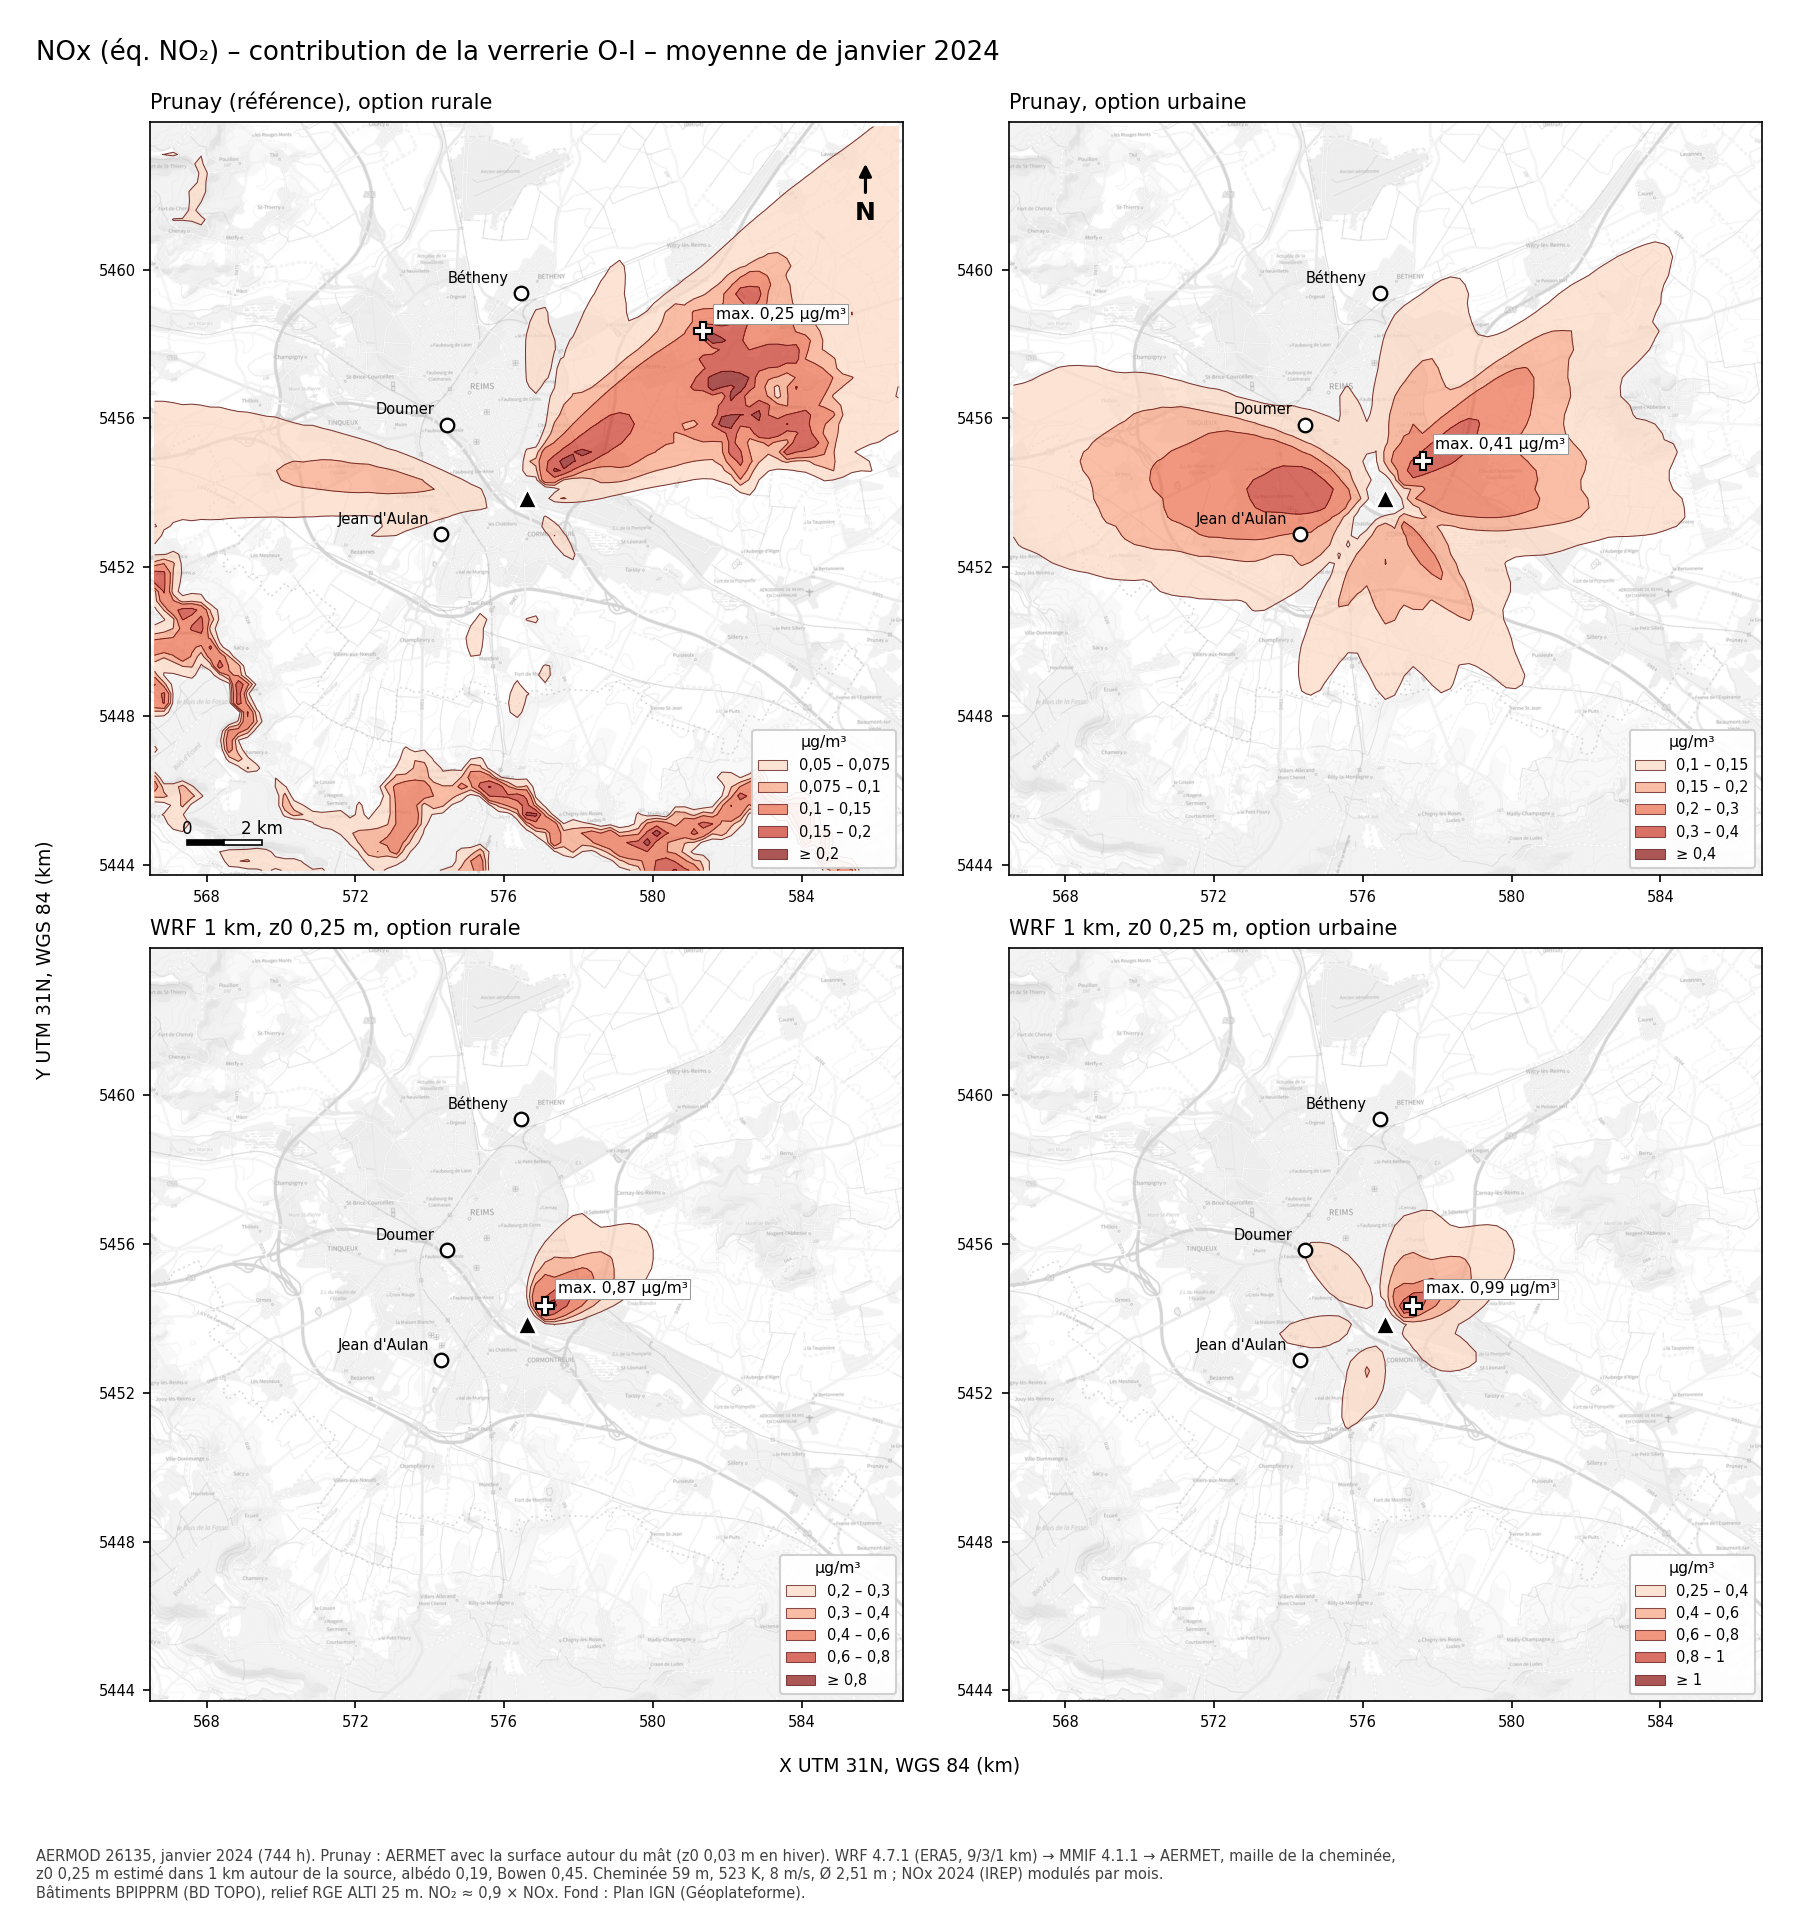
\includegraphics[width=0.70\textwidth]{etape8_janvier_moyenne.png}
\caption{Moyenne de janvier 2024 (\NOx)~: Prunay (haut) et WRF avec \zz{}~=~0,25~m (bas), options rurale et urbaine.
Chaque carte a ses propres classes.}
\end{figure}

\section{Autres sources d'incertitude}
\begin{table}[htbp]
\centering\small
\caption{Effet de chaque hypothèse testée séparément.}
\begin{tabularx}{\textwidth}{lY}
\toprule
Hypothèse & Effet \\
\midrule
Rural ou urbain & facteur dominant~: stations × 2 à × 4,6~; maximum horaire $-72$~\% \\
Météo simulée (WRF, 1~km) & stations × 1,2 à × 5,7 en hiver, × 0,6 à × 1 en été~; toujours $\leq$ 0,26~\ugm{} \\
Rugosité de Prunay portée à 0,25~m & + 18 à 20~\% aux stations \\
Température des fumées ± 50~°C & ± 10 à 20~\% \\
Émissions déclarées & proportionnel \\
Diamètre, position, bâtiments, découpage horaire & < 7~\% \\
Rayonnement mesuré au lieu de la nébulosité & + 8 à 12~\% au maximum annuel, 0 à + 6~\% aux stations \\
Brouillard (112~h en 2024) & contribution rurale quasi nulle pendant le brouillard \\
Fumigation matinale (AERSCREEN) & 6,5~\ugm{} sur 1~h à 9,3~km, sous les autres maxima horaires \\
\bottomrule
\end{tabularx}
\end{table}

\textbf{Rayonnement.} AERMET estime le rayonnement à partir de la nébulosité (Kasten et Czeplak, 1980). Comparé au
rayonnement global mesuré à Prunay, il est juste en moyenne ($-9$~\%, $r = 0{,}86$), mais il sous-estime de 32~\% les
journées couvertes. Recalculer la nébulosité à partir du rayonnement mesuré change peu les résultats.

\textbf{Brouillard.} Pendant les 112~heures de brouillard de 2024, AERMET décrit une couche limite stable et peu
épaisse (couche mélangée de 67~m). Le \NOx{} mesuré est alors 2 à 3,5 fois plus élevé, à cause du trafic qui
s'accumule. Le panache, plus haut, ne touche pas le sol en option rurale. Petite anomalie~: 14~\% de ces heures
sont vues par AERMET comme un ciel clair.

\textbf{Fumigation.} Le matin, quand l'inversion se dissipe, un panache resté en altitude peut être rabattu d'un
coup vers le sol. AERMOD ne simule pas ce phénomène. AERSCREEN, l'outil de dépistage de l'EPA (méthode de Turner,
1970), situe cette fumigation à 9,3~km. Le panache a alors eu le temps de s'élargir, et la concentration ne dépasse
pas 6,5~\ugm.

\section{Volet sanitaire}
Pour les 173 établissements sensibles situés à moins de 4~km (BD TOPO), la contribution de la verrerie au \NOd{} est
au plus de 0,10 à 0,19~\ugm{} en moyenne annuelle, 2,1~\ugm{} sur 24~h et 11~\ugm{} sur 1~h. En retenant la plus
défavorable des deux options, le quotient de danger de la verrerie est inférieur ou égal à 0,02 en moyenne annuelle
(valeur guide de l'OMS, 10~\ugm) et à 0,06 sur 1~h (200~\ugm). L'exposition totale, environ 9,5~\ugm, est dominée
par le fond urbain.

\section{Limites et perspectives}
\begin{itemize}
\item \textbf{Émissions}~: seul le total annuel déclaré est connu, réparti par mois selon la production. Les débits
horaires réels et la marche dégradée (cheminées de secours) ne sont pas représentés.
\item \textbf{Paramètres de cheminée}~: valeurs prescrites par l'arrêté (vitesse minimale, débit nominal), et non
mesurées.
\item \textbf{Rural ou urbain}~: la question reste ouverte. Les mesures défavorisent l'option urbaine sans la
réfuter, et les critères de l'EPA se contredisent.
\item \textbf{Météo}~: Prunay est à 7~km, et WRF n'a été exécuté que sur deux mois. Une année complète demanderait
environ 18~jours de calcul.
\item \textbf{Validation}~: les stations, à 2,5–5,5~km, ne peuvent pas trancher. Des tubes passifs non plus~:
l'apport de l'usine sur 14~jours (0,1 à 0,8~\ugm{} à 0,5–1~km) est bien inférieur à leur incertitude (± 3 à
4~\ugm). Une validation demanderait des analyseurs horaires de \NOx{} et de \SOd{} et un anémomètre à 0,5–1~km au
nord-est, avec les émissions horaires réelles de la cheminée.
\end{itemize}

\section{Conclusions}
\begin{enumerate}
\item La verrerie contribue pour moins de 0,5~\% (option rurale) à 1,4~\% (option urbaine) du \NOd{} moyen
mesuré aux stations de Reims. Le \NOd{} urbain est dominé par le trafic et par les situations météorologiques
stagnantes.
\item Le réseau ne voit pas l'usine directement. Treize ans de mesures défavorisent l'option urbaine sans la réfuter.
\item Le choix rural ou urbain est la principale source d'incertitude. Aucun autre facteur testé ne change l'ordre
de grandeur.
\item L'usine ne compte qu'à proximité (moins de 1~km au nord-est) et, certaines heures, sur le relief. Le risque
sanitaire associé à sa contribution est faible.
\end{enumerate}

\section{Données et code}\label{sec:repro}
Dépôt~: \url{https://github.com/Mahamat-A/aermod-reims-verrerie} (entrées AERMET, AERMAP, AERMOD, MMIF et AERSCREEN,
scripts Python, figures, rapports détaillés par étape). Logiciels~: AERMOD 26135, AERMET, AERMAP 24142, BPIPPRM,
AERSCREEN 21112 (EPA), MMIF 4.1.1, WRF 4.7.1. Les données des producteurs restent soumises à leurs conditions
(NOAA, Météo-France, IGN, LCSQA, AEE, Copernicus).

\section*{Références}
\small
\begin{description}[leftmargin=0pt,labelindent=0pt,itemsep=1pt,font=\normalfont]
\item Auer, A.\,H. (1978). Correlation of land use and cover with meteorological anomalies. \textit{Journal of
Applied Meteorology}, 17, 636–643.
\item Cimorelli, A.\,J. et al. (2005). AERMOD: A dispersion model for industrial source applications. Part I:
General model formulation and boundary layer characterization. \textit{Journal of Applied Meteorology}, 44, 682–693.
\item Hersbach, H. et al. (2020). The ERA5 global reanalysis. \textit{Quarterly Journal of the Royal Meteorological
Society}, 146, 1999–2049.
\item Kasten, F. et Czeplak, G. (1980). Solar and terrestrial radiation dependent on the amount and type of cloud.
\textit{Solar Energy}, 24, 177–189.
\item Paine, R., Warren, L.\,L. et Moore, G.\,E. (2016). Source characterization refinements for routine modeling
applications. \textit{Atmospheric Environment}, 129, 55–67. doi:10.1016/j.atmosenv.2016.01.003.
\item Skamarock, W.\,C. et al. (2019). \textit{A description of the Advanced Research WRF Model Version 4}. NCAR
Technical Note NCAR/TN-556+STR.
\item Turner, D.\,B. (1970). \textit{Workbook of Atmospheric Dispersion Estimates}. US Public Health Service,
publication 999-AP-26.
\item U.S. EPA (2021). \textit{AERSCREEN User's Guide}. EPA-454/B-21-005.
\item U.S. EPA (2024). \textit{Guidance on the Use of the Mesoscale Model Interface Program (MMIF) for AERMOD
Applications}. EPA-454/B-24-005.
\item U.S. EPA (2026). \textit{User's Guide for the AMS/EPA Regulatory Model (AERMOD)}. EPA-454/B-26-001.
\item U.S. EPA (2026). \textit{User's Guide for the AERMOD Meteorological Preprocessor (AERMET)}. EPA-454/B-26-005.
\end{description}

\end{document}
